\documentclass[12pt]{article}
\usepackage{fontspec}   %加這個就可以設定字體
\usepackage{xeCJK}       %讓中英文字體分開設置
\setmainfont{Times New Roman}
\setCJKmainfont{標楷體} %設定中文為系統上的字型,而英文不去更動,使用原TeX字型
\XeTeXlinebreaklocale "zh"             %這兩行一定要加,中文才能自動換行
\XeTeXlinebreakskip = 0pt plus 1pt     %這兩行一定要加,中文才能自動換行
\usepackage{amsmath, amsthm, amssymb} %引入數學符號的套件,例如實數R、定理Thm...
\usepackage{graphicx}                 %現在, 假設我們要插入 pic.png 這個圖檔, 使用
%\title{我是標題}
%\author{我是作者}
%\date{} %不要日期

\newcommand{\uA}       {\mbox{\boldmath$A$}}
\usepackage{textcomp}
\usepackage{array}
\usepackage{graphicx}
\usepackage{colortbl}
\usepackage{color,xcolor}
\usepackage{listings}
\usepackage{array,booktabs}   %這三個為表格使用的套件
\usepackage{textpos}
\usepackage{float}
\usepackage{listings}

\title{Statistical learning assignment 2 - chapter 2}
\author{孫浩哲 \hspace{0.7cm} M072040002}
\date{September 27, 2018}
\begin{document}
\maketitle
\ \\
%%%%%%%%%%%%%%%%%%%%%%%%%%%%%%%%%%%%%%%%%%%%%%%%%%
\Large{1.}
\normalsize
\begin{itemize}
\item[\normalsize(a)]
better, because a more flexible way will fit the large sample size better.
\item[(b)]
worse, it might overfitting.
\item[(c)]
better, the more parameters, the more degree of freedom, a flexible model can fit the data well.
\item[(d)]
worse, if we use more flexible model on the situation, it might increase variance.
\end{itemize}
%%%%%%%%%%%%%%%%%%%%%%%%%%%%%%%%%%%%%%%%%%%%%%%%%%
\Large{2.}
\begin{itemize}
\item[\normalsize(a)]
\normalsize regression, inference.\\[2ex]
Because the CEO salary is quantitative output and we want to know the relationship between two features, so we use regression to make the inference.\\[2ex]
n - $500$ firms in the US.\\
p - profit, number of employees, industry.
\item[(b)]
classification, prediction.\\[2ex]
The "success" and "failure" is a qualitative output and we want to predict new product's success or failure, so we use classification to make the prediction.\\[2ex]
n - $20$ similar products previously launched.\\
p - price charged, marketing budget, comp. price, ten other variables.
\item[(c)]
regression, prediction.\\[2ex]
The percentage of change in US dollar is quantitative output and we want to make a prediction, so we use regression to make the prediction.\\[2ex]
n - $52$ weeks of $2012$ weekly data.\\
p - $\%$ change in US market, $\%$ change in British market, $\%$ change in German market.
\end{itemize}
%%%%%%%%%%%%%%%%%%%%%%%%%%%%%%%%%%%%%%%%%%%%%%%%%%
\Large{3.}
\normalsize
\begin{itemize}
\item[(a)]
\ \\
\centerline{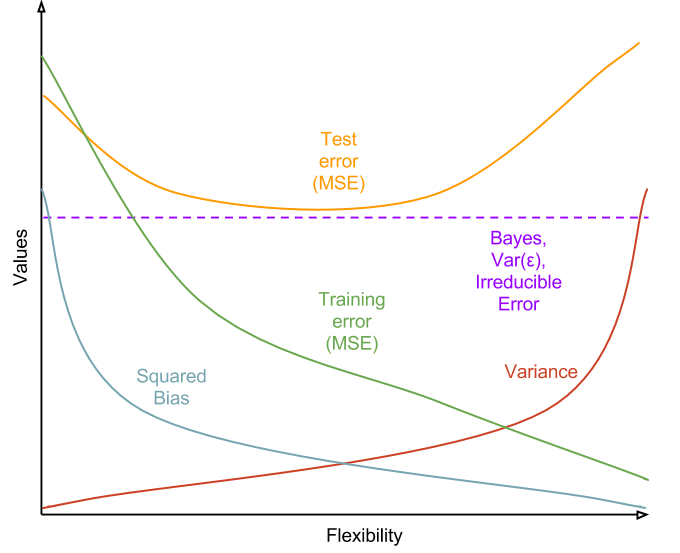
\includegraphics[width=1.0\linewidth]{bias-variance-decomposition}}
\item[(b)]
Because each index is larger than $0$, so each of five curves has the shape displayed in the figure.
\end{itemize}
%%%%%%%%%%%%%%%%%%%%%%%%%%%%%%%%%%%%%%%%%%%%%%%%%%
\Large{4.}
\normalsize
\begin{itemize}
\item[(a)]
i. Iris dataset\\
Response:Setosa, Versicolor, Virginica\\
Predictors:length and width of sepal and petal.\\
$\bullet$ Prediction.Because we want to predict the species of iris.\\[2ex]
ii. Race\\
Response:European, Asian, American, African\\
Predictors:height, weight, complexion.\\
$\bullet$ Prediction.We want to classify the race.\\[2ex]
iii. Stock market price direction\\
Response:up, down\\
Predictors:price movement of each day in last week\\
$\bullet$ Prediction.We just predict the Stock market price direction is up or down.
\item[(b)]
i. Salary\\
Response:Salary\\
Predictors:years of education, industry experience, Nature of the work\\
$\bullet$ Inference.We build the function to explore the relationship between the features. \\[2ex]
ii. House price\\
Response:House price\\
Predictors:region, population, GDP\\
$\bullet$ Inference.Reason is the same as (i.).\\[2ex]
iii. Test score\\
Response:Test score\\
Predictors:reading time\\
$\bullet$ Inference.Reason is the same as (i.).
\item[(c)]
i. Cancer type.\\
ii. City or country.\\
iii. Youtube video recommendations.
\end{itemize}
\newpage
%%%%%%%%%%%%%%%%%%%%%%%%%%%%%%%%%%%%%%%%%%%%%%%%%%
\Large{5.}
\normalsize
\begin{itemize}
\item[i.]
\ \\
Advantages:Obtaining a better fit for non-linear models, decreasing bias.\\[3ex]
Disadvantages:Large number of parameters, overfitting, increasing variance.
\item[ii.]
\ \\
When we are interested in prediction and not the interpretability of the results.
\item[iii.]
\ \\
When we are interested in inference and the interpretability of the results.
\end{itemize}
\end{document} 